\subsection{بخش ب}
در این بخش با استفاده از بهینه‌سازی مقادیر اولیه
$\theta$
و
$\psi$
محاسبه شد. مقادیر
$\theta_0$،
$\psi_0$ 
و فاصله ازدست‌دهی\LTRfootnote{Miss Distance} آورده شده است.

\begin{table}[H]
	\caption{شرایط اولیه و فاصله ازدست‌دهی }
	\centering
	\begin{tabular}{cc}
		\hline
		 Value &  Parameter \\
		\hline
		\lr{\ang{39.9892}} & \lr{$\theta_0$}\\
		\lr{\ang{0}}  & $\psi_0$ \\ 
		\lr{0.0741}& \lr{Miss Distance(m)}  \\
		\hline
	\end{tabular}
	
	\label{tab:4gps_solve}
\end{table}
برای اعمال شتاب در دو ثانیه آخر از زمان نهایی شبیه‌سازی بالا استفاده شده و سپس دو ثانیه از آن کم شد و در نهایت شبیه‌سازی با شرایط جدید انجام شد. با در نظر گرفتن اعمال شتاب در دو ثانیه، فاصله ازدست‌دهی جدید برابر با ۲۲/۵ متر شد. 

نتایج شبیه‌سازی در دو حالت اشاره شده در پایین آورده شده است.

\begin{figure}[H]
	\centering
	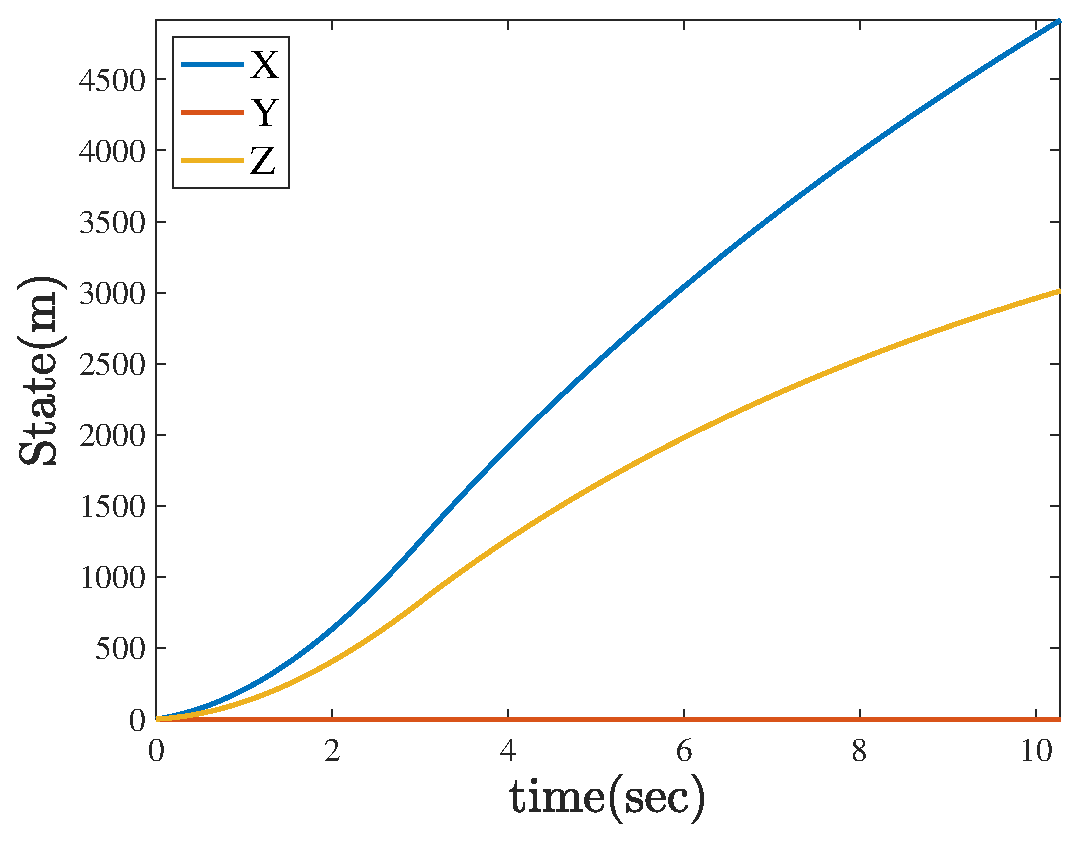
\includegraphics[width=.75\linewidth]{../Figure/b/missle_state}
	\caption{موقعیت موشک با شرایط اولیه بهینه شده}
\end{figure}

\begin{figure}[H]
	\centering
	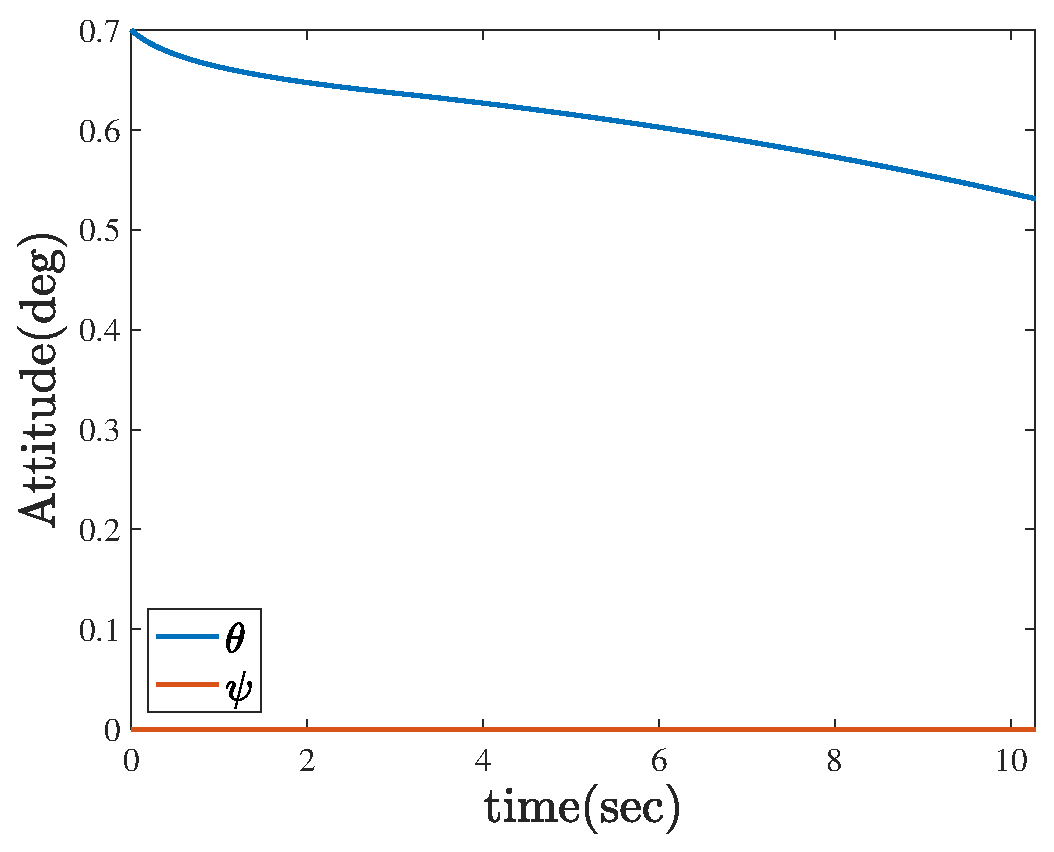
\includegraphics[width=.75\linewidth]{../Figure/b/missle_attitude}
	\caption{وضعیت موشک با شرایط اولیه بهینه شده}
\end{figure}

\begin{figure}[H]
	\centering
	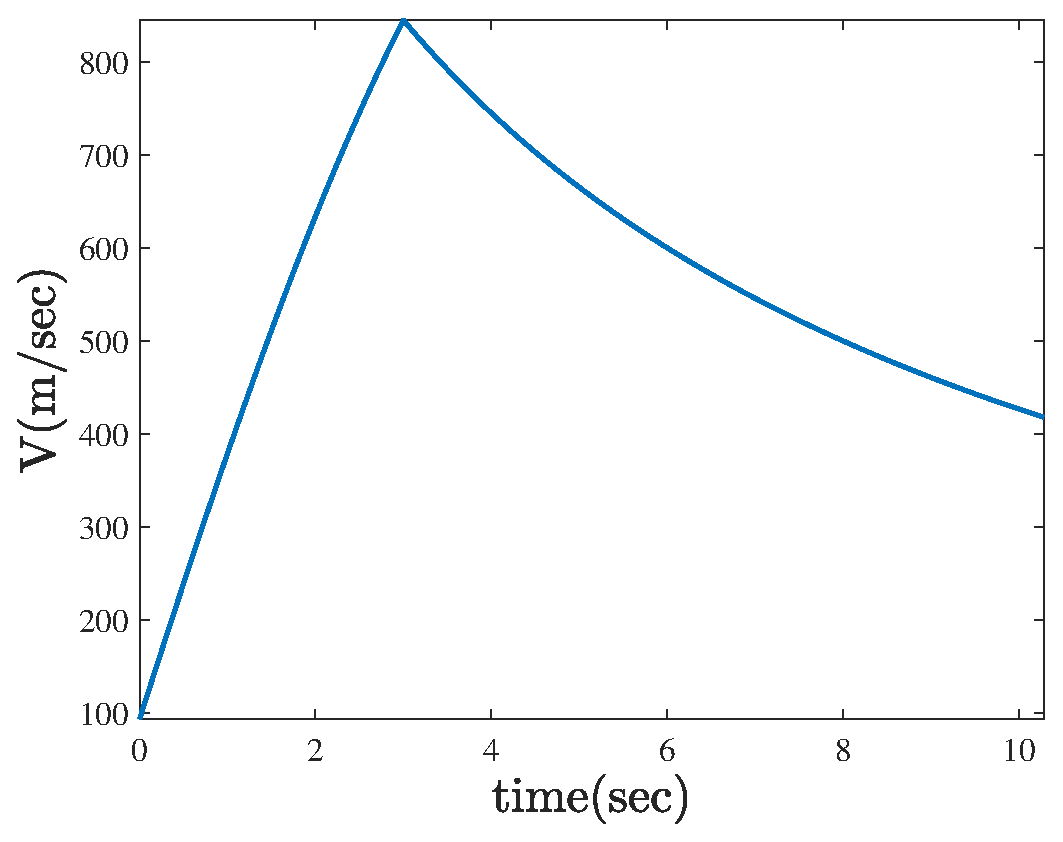
\includegraphics[width=.75\linewidth]{../Figure/b/missle_V}
	\caption{سرعت موشک با شرایط اولیه بهینه شده}
\end{figure}

\begin{figure}[H]
	\centering
	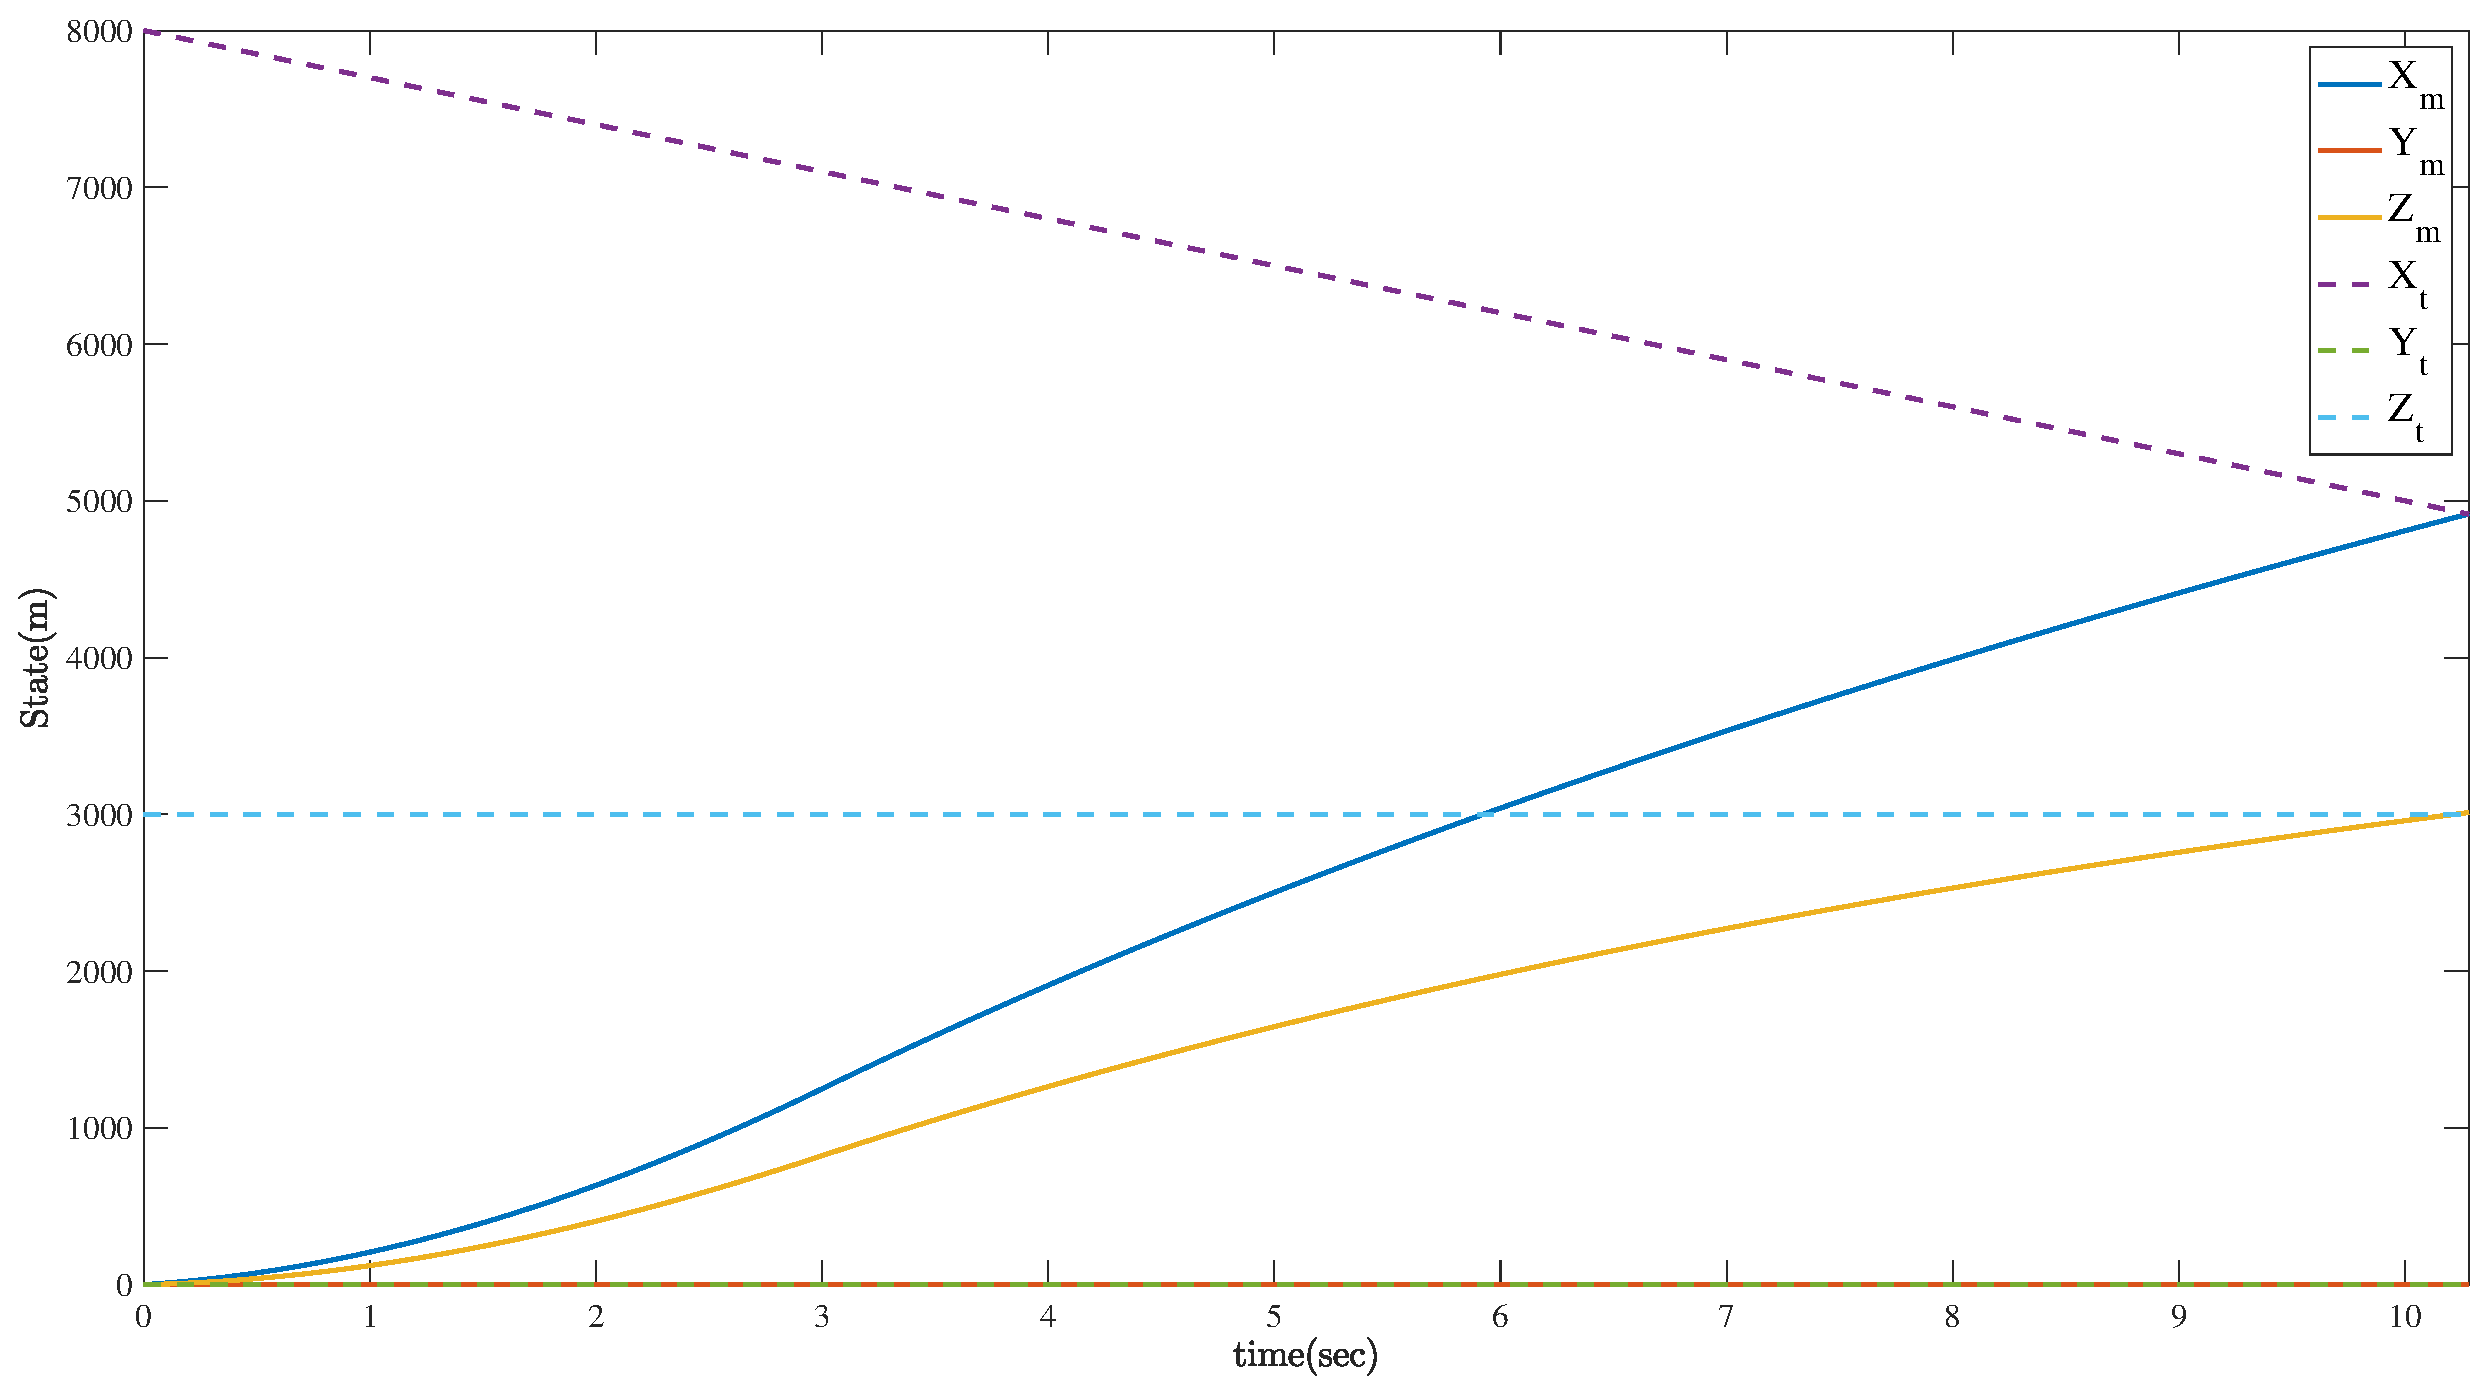
\includegraphics[width=\linewidth]{../Figure/b/missle_vs_target_state}
	\caption{موقعیت موشک و هدف با شرایط اولیه بهینه شده}
\end{figure}

\begin{figure}[H]
	\centering
	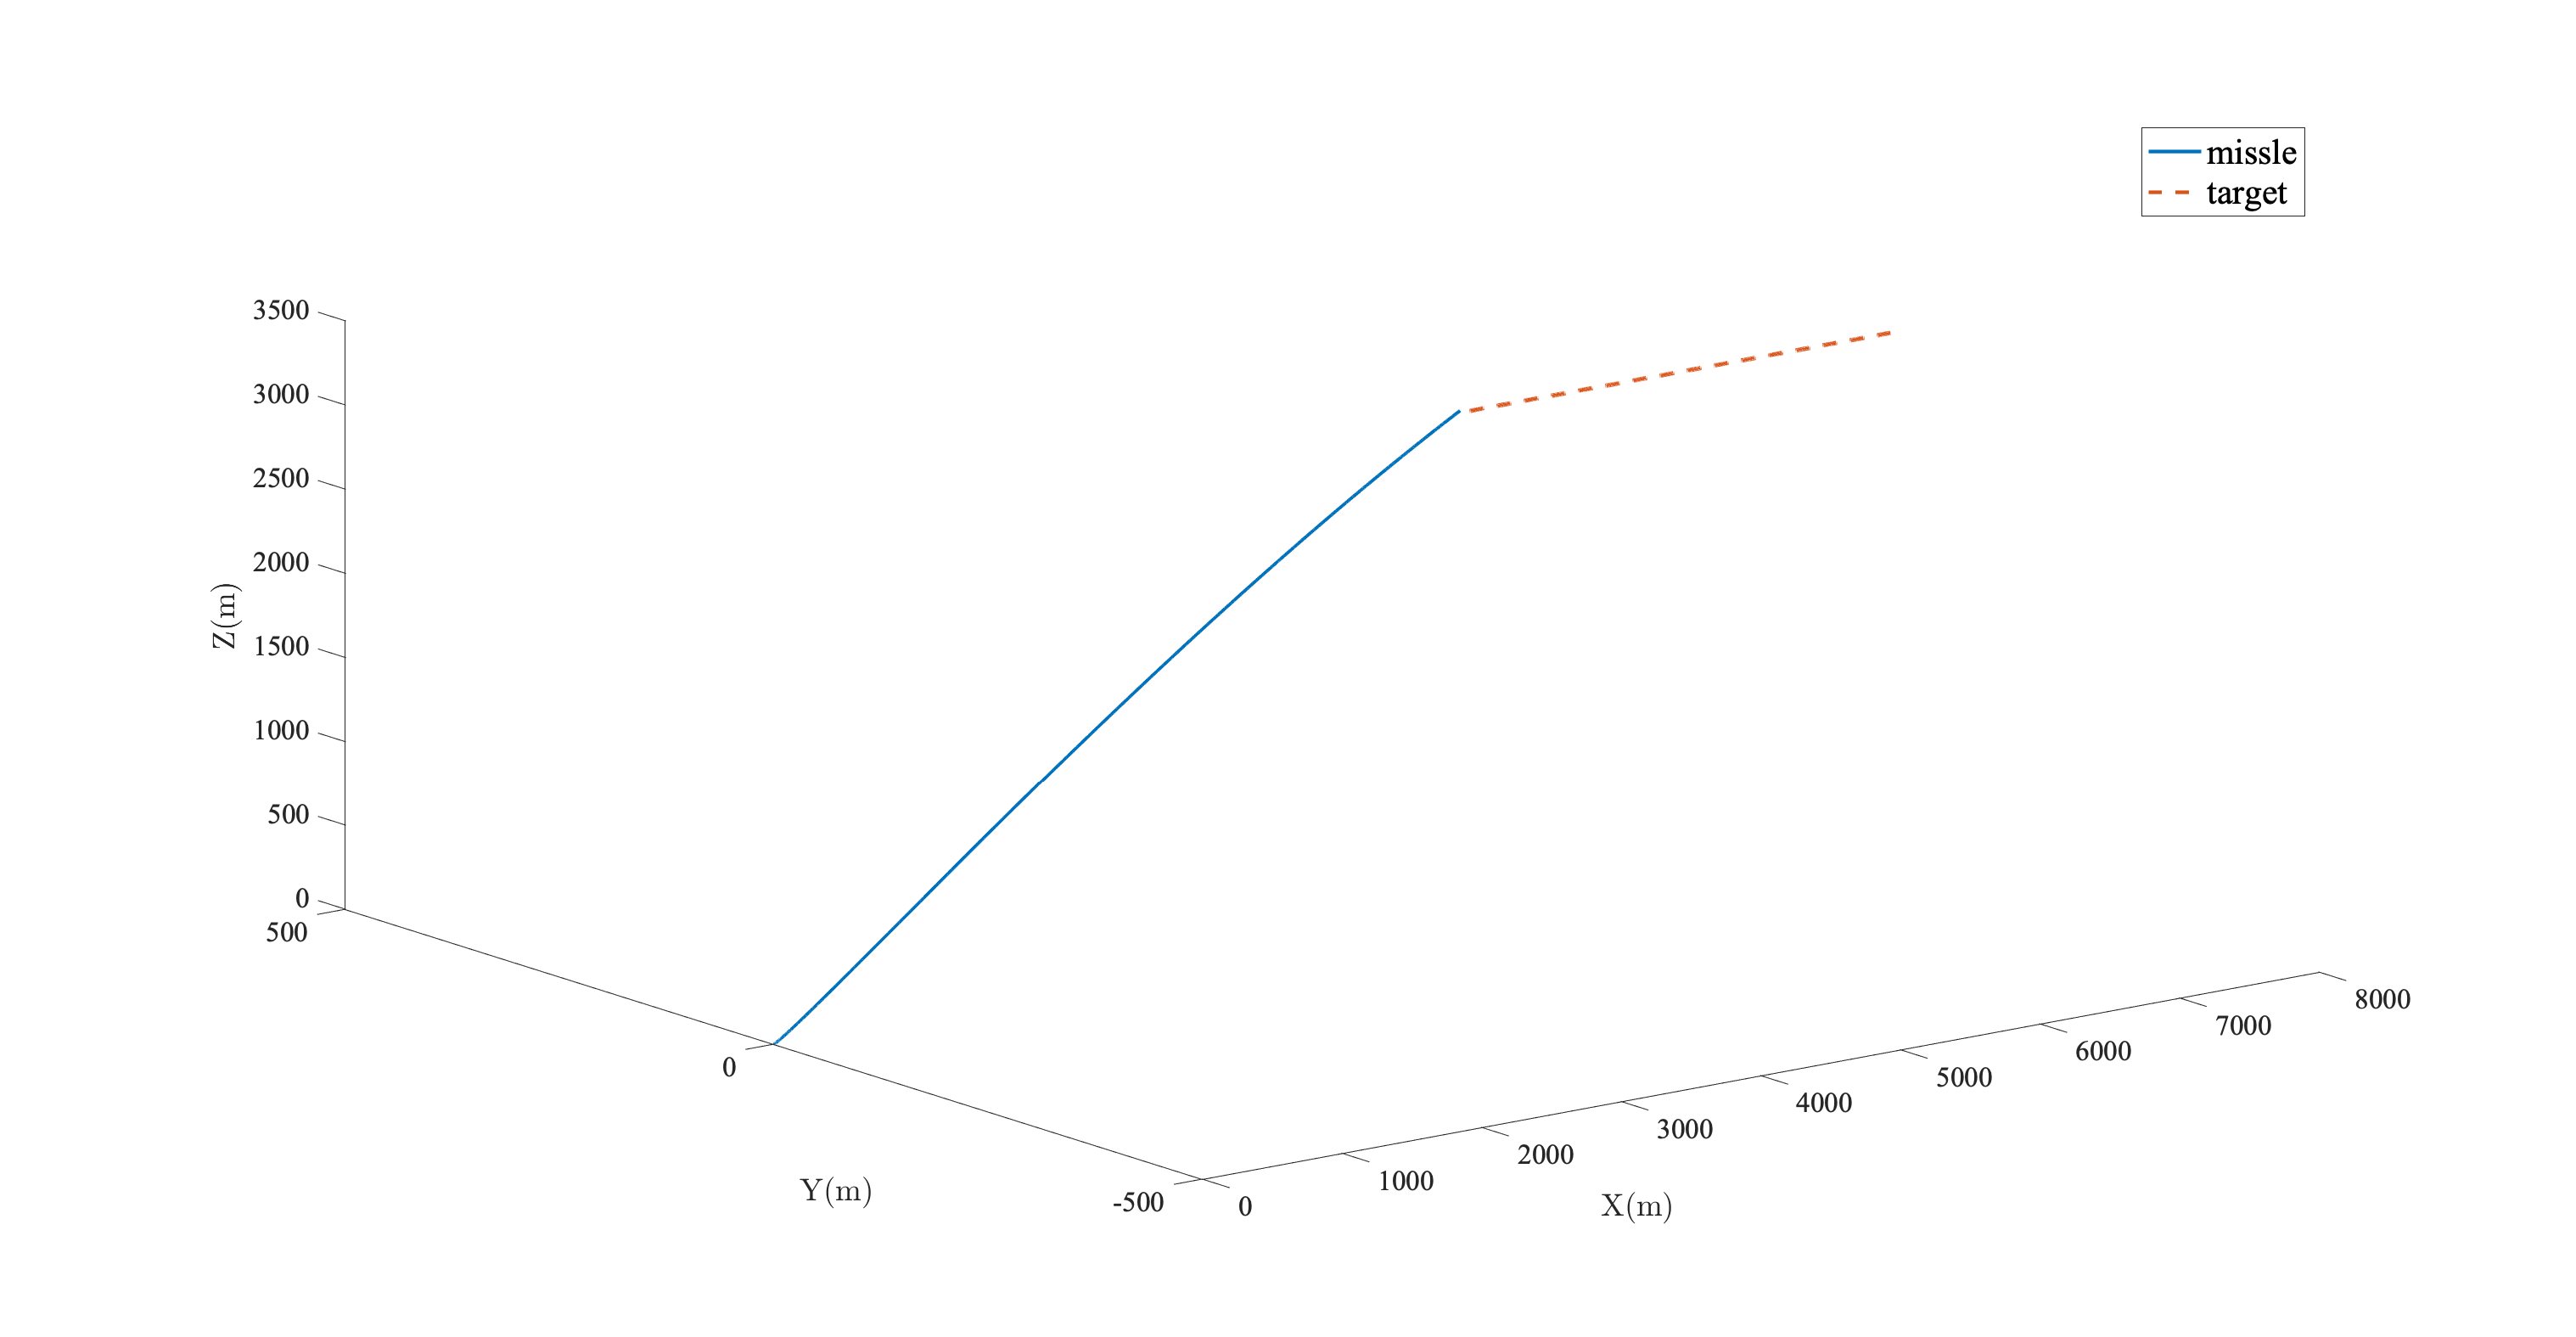
\includegraphics[width=\linewidth]{../Figure/b/3DoF_missle_vs_target_state}
	\caption{موقعیت موشک و هدف به صورت سه بعدی با شرایط اولیه بهینه شده}
\end{figure}

\begin{figure}[H]
	\centering
	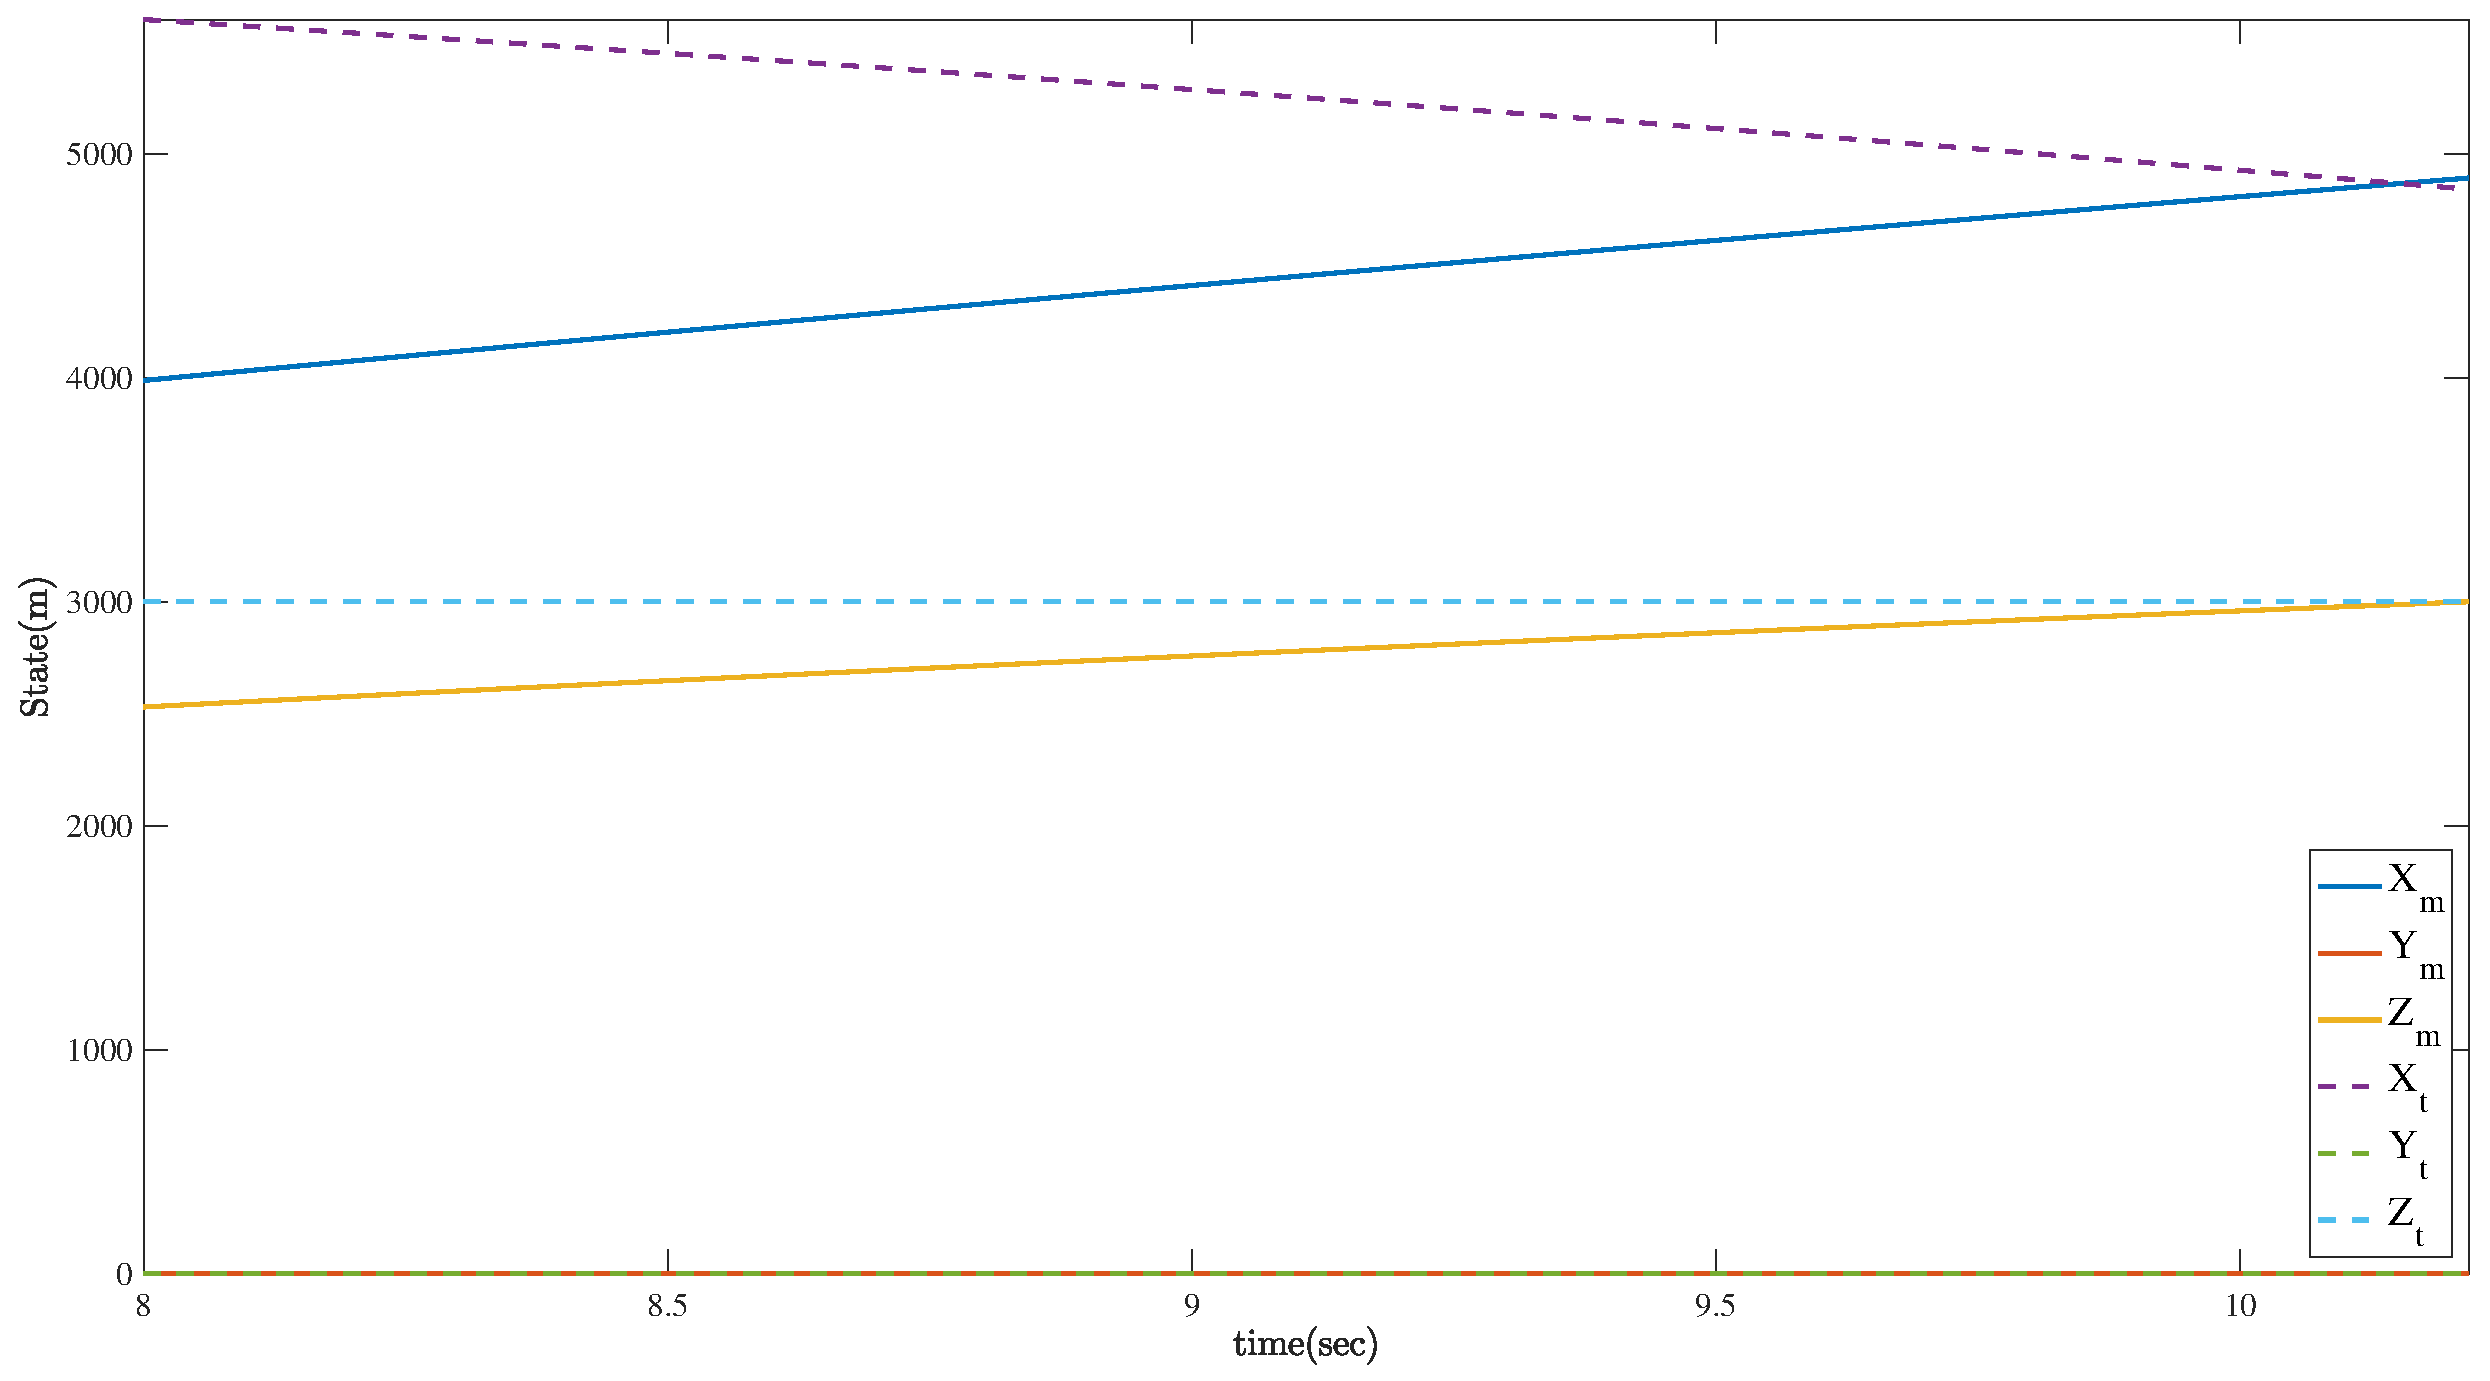
\includegraphics[width=\linewidth]{../Figure/b/missle_vs_target_state_maneuver}
	\caption{موقعیت موشک و هدف با شرایط اولیه بهینه شده همراه با مانور هدف}
\end{figure}

\begin{figure}[H]
	\centering
	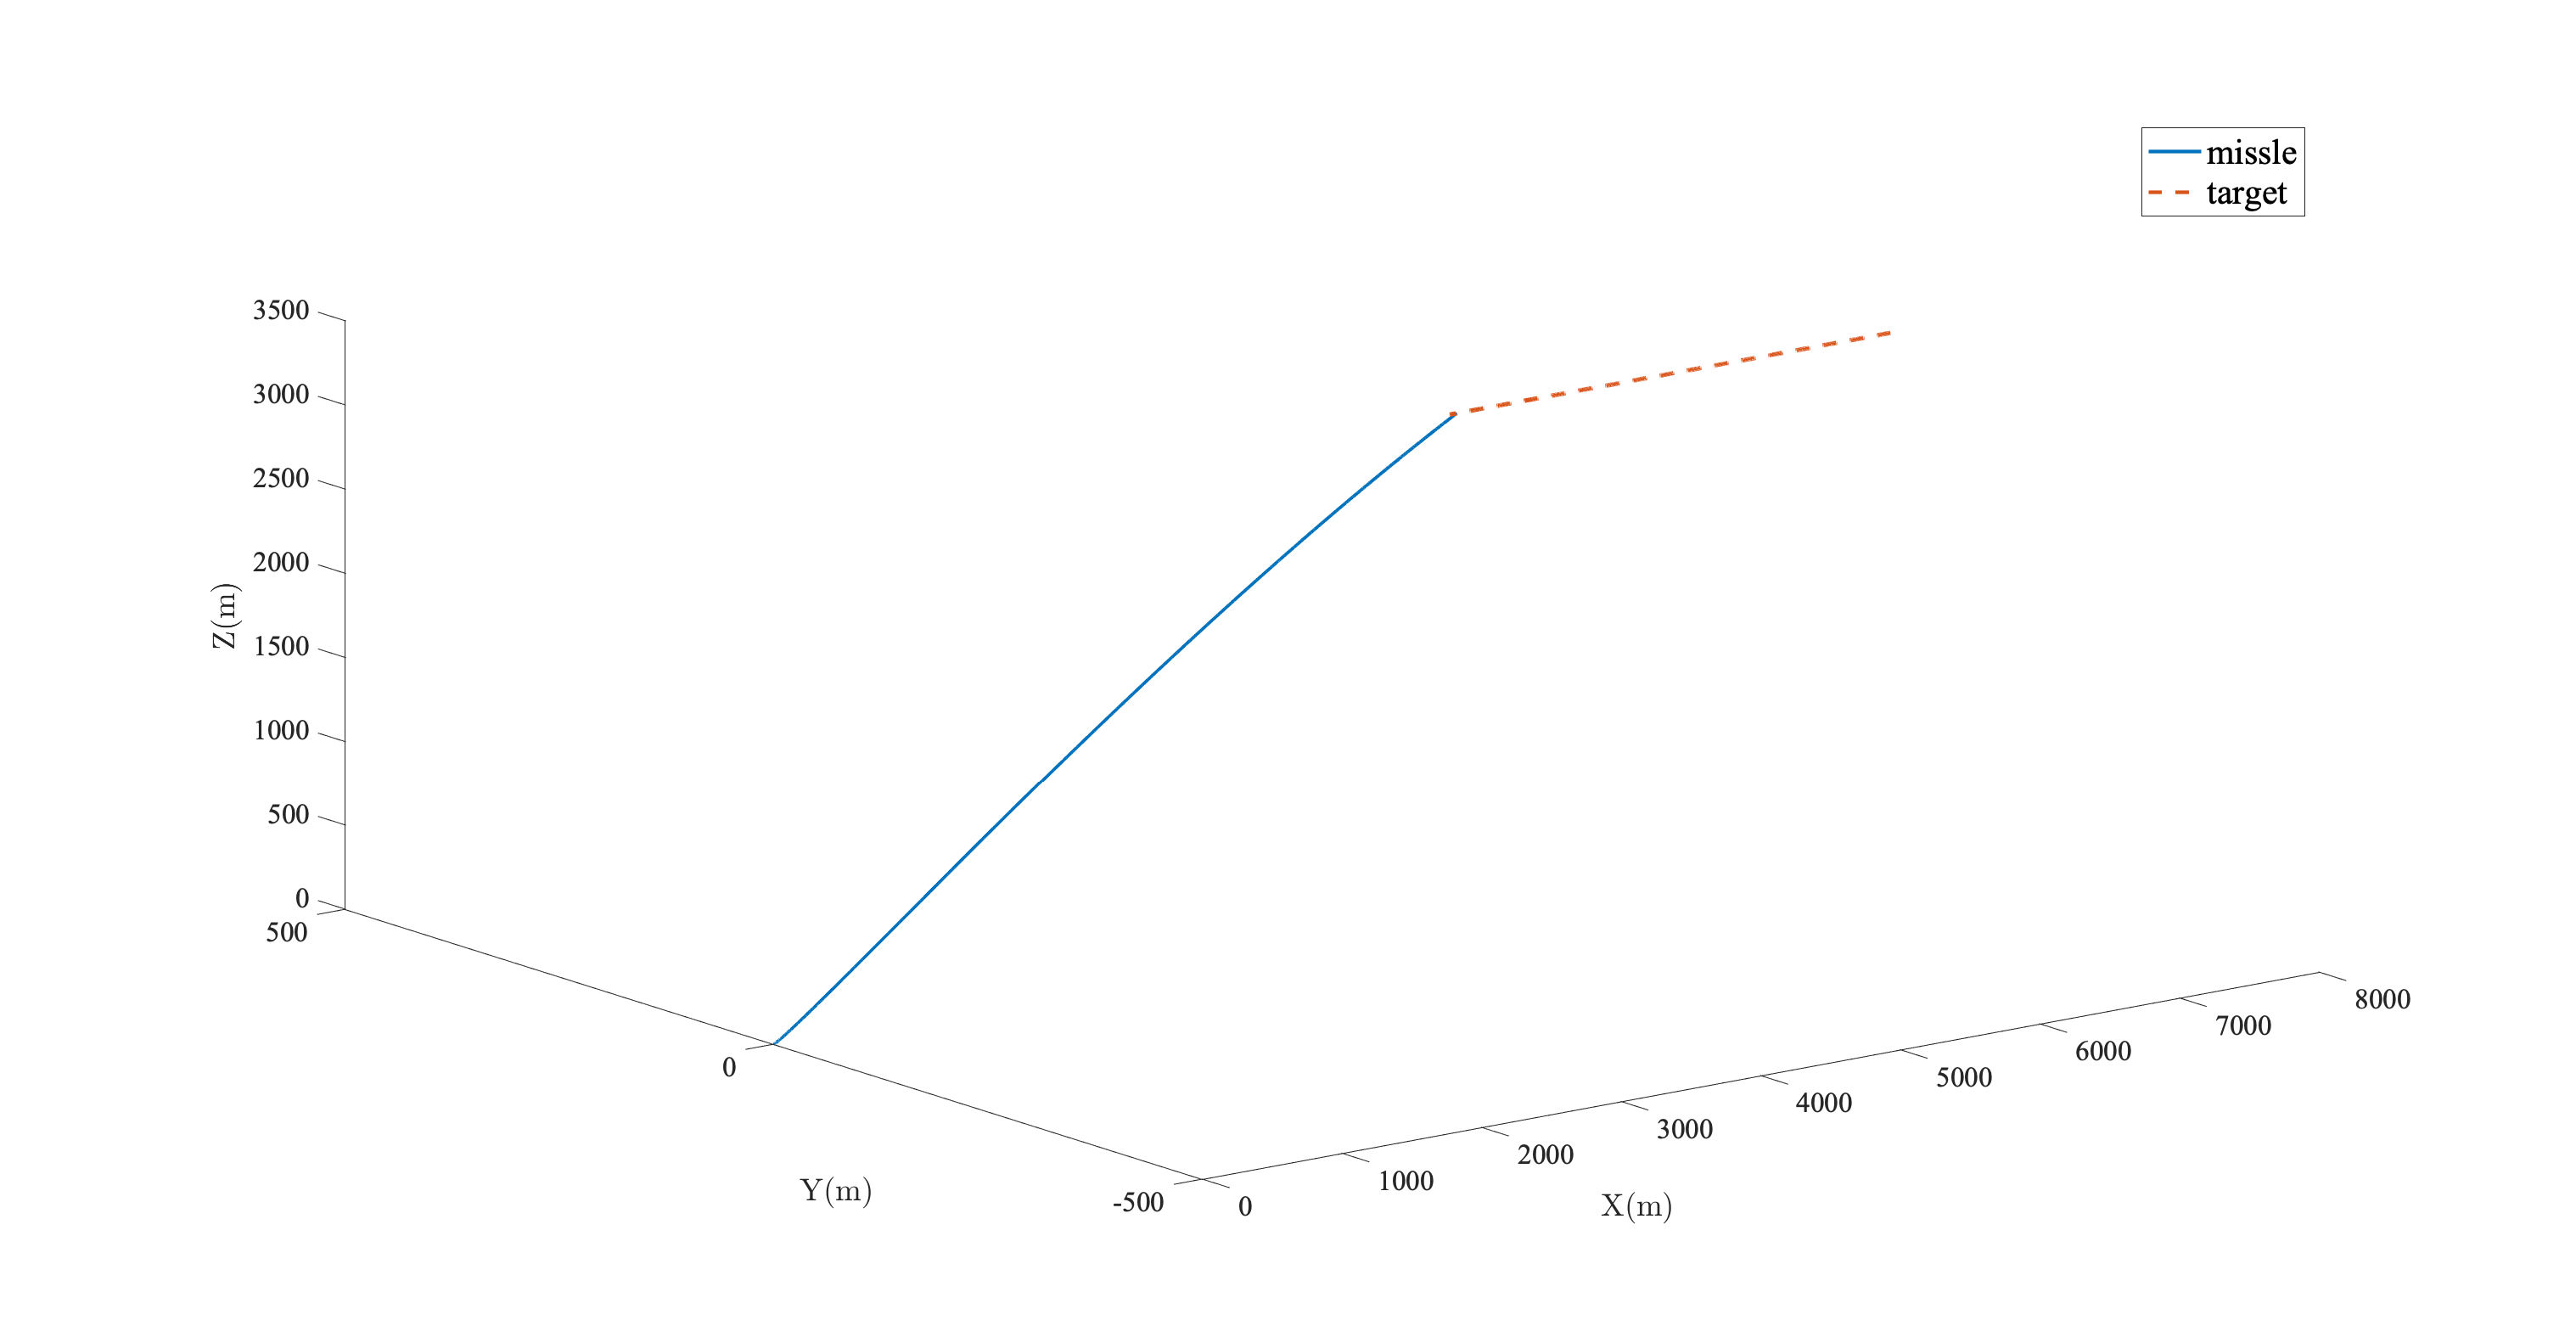
\includegraphics[width=\linewidth]{../Figure/b/3DoF_missle_vs_target_state_maneuver}
	\caption{موقعیت موشک و هدف به صورت سه بعدی با شرایط اولیه بهینه شده همراه با مانور هدف}
\end{figure}

